\section{Determination of $\rho$}
\label{sec:rho}

The value of the $\rho$ parameter can be extracted from the differential cross-section thanks to the effects of Coulomb-nuclear interference (CNI). Our modelling of these effects is summarised in Section \ref{sec:rho cni}, and Section \ref{sec:rho anal} describes data fits and results.

%----------------------------------------------------------------------------------------------------
\subsection{Coulomb-Nuclear Interference}
\label{sec:rho cni}

A detailed overview of different CNI descriptions was given in Ref.~\cite{totem-8tev-1km}, Section 6. Here we briefly summarise the choices used for the presented analysis.

The Coulomb amplitude can be derived from QED. In the one-photon approximation it yields the cross-section
\begin{equation}
\label{eq:coul cs}
	{\d\sigma^{\rm C}\over \d t} = {4\pi\alpha^2\over t^2}\,{\mathcal{F}}^4\ ,
\end{equation}
where $\alpha$ is the fine-structure constant and $\mathcal{F}$ represents an experimentally determined form factor. Several form factor determinations have been considered (by Puckett et al., Arrington et al.~and Borkowski et al., see summary in \cite{elegent}) and no difference in results has been observed.

Motivated by the observed differential cross-section, at low $|t|$ the modulus of the nuclear amplitude is parametrised as
\begin{equation}
\label{eq:nuc mod}
\left | {\cal A}^{\rm N}(t) \right | = \sqrt{s\over\pi} {p\over \hbar c} \sqrt{a} \exp\left( {1\over 2} \sum\limits_{n = 1}^{N_b} b_n\, t^n \right)\ .
\end{equation}
The $b_1$ parameter is responsible for the leading exponential decrease, the other $b_n$ parameters can describe small deviations from the leading behaviour. Since the calculation of CNI may, in principle, involve integrations (e.g.~Eq.~(\ref{eq:int kl})), it is necessary to extend the nuclear amplitude meaningfully to higher $|t|$ values, too. In that region, the amplitude is fixed to a function that describes well the dip-bump structure observed in the data, see the red curve in Figure~\ref{fig:high t desc}. In order to avoid numerical problems, the intermediate $|t|$ region is modelled with a continuous and smooth interpolation between the low and high-$|t|$ parts. It has been checked that altering the high-$|t|$ part within reasonable limits has negligible impact on the results.

\begin{figure*}
\vskip-5mm
\begin{center}
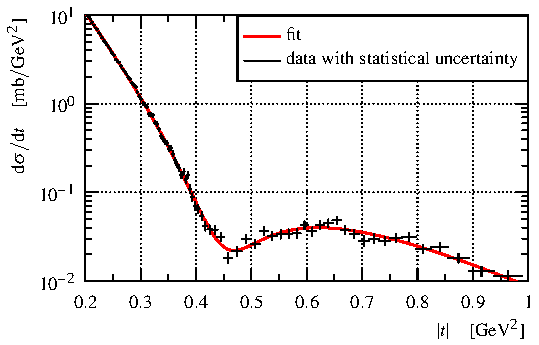
\includegraphics{fig/high_t_description.pdf}
\caption{%
Differential cross-section at higher $|t|$ values as determined in the ``2RP'' analysis (black points) with a fit (red line) used for the evaluation of the CNI effects. The fit also allows for a first dip-bump characterisation at $13\un{TeV}$: the dip is located at $|t| \approx 0.47\un{GeV^2}$, the bump at $|t|\approx 0.62\un{GeV^2}$ and the bump/dip cross-section ratio is about $1.8$. A precise quantification will be given in a forthcoming TOTEM publication using a dedicated high-statistics dataset. For comparison: at $7\un{TeV}$ the dip was found at $0.53\un{GeV^2}$ and the bump/dip ratio $\lesssim 1.7$ \cite{totem-7tev-first}.
}
\label{fig:high t desc}
\end{center}
\end{figure*}

Several parametrisations have been considered for the phase of the nuclear amplitude. Since one of the main goals of this analysis is to compare the newly obtained $\rho$ value with those at lower energies, we have focused on parametrisations similar to past analyses. Consequently we have considered phases with slow variation at low $|t|$: constant, Bailly and standard from \cite{totem-8tev-1km}. No dependence of the results on this choice was observed and therefore only the constant phase
\begin{equation}
\label{eq:nuc phase con}
\arg {\cal A}^{\rm N}(t) = {\pi\over 2} - \arctan\rho = \hbox{const} \ .
\end{equation}
will be retained in what follows. A more complete exploration including phases leading to a peripheral description of elastic scattering is planned for a forthcoming TOTEM publication.

We have used the most general interference formula available in the literature -- the ``KL'' formula \cite{kl94}:
\begin{equation}
\label{eq:int kl}
	\begin{aligned}
		{\d\sigma\over \d t}^{\rm C+N} =& {\pi (\hbar c)^2 \over s p^2} \left | {\alpha s\over t} {\cal F}^2
			+ {\cal A}^{\rm N}\, \Big[1 - \I\alpha G(t)\Big] \right |^2\ ,\cr
		G(t) =& \int\limits_{-4p^2}^0 \d t'\, \log {t'\over t} {\d\phantom{t'}\over \d t'} {\cal F}^2(t')
			  - \int\limits_{-4p^2}^0 \d t' \left( {{\cal A}^{\rm N}(t') \over {\cal A}^{\rm N}(t)} - 1 \right) { I(t, t')\over 2\pi }\ , \cr
		I(t, t') =& \int_0^{2\pi} \d\phi\ {{\cal F}^2(t'')\over t''}\ ,\cr
		t'' =& t + t' + 2\sqrt{t\, t'} \cos\phi\ ,\cr
	\end{aligned}
\end{equation}
which is numerically almost identical to the formula by Cahn \cite{cahn82} as shown in \cite{totem-8tev-1km}. The CNI effects were calculated by the computer code from Ref.~\cite{elegent}.


%----------------------------------------------------------------------------------------------------
\subsection{Data fits}
\label{sec:rho anal}

The fits have been carried out with the standard least-squares method, minimising
\begin{equation}
\label{eq:chi sq A}
	\chi^2 = \Delta^\T \mat V^{-1} \Delta\ ,\quad
	\Delta_i = \left.{\d\sigma\over \d t}\right|_{{\rm bin}\ i} - {\d\sigma^{\rm C+N}\over\d t}\left(t^{\rm rep}_{{\rm bin}\ i}\right)\ ,\quad
	\mat V = \mat V_{\rm stat} + \mat V_{\rm syst}\ ,\
\end{equation}
where $\Delta$ is a vector of differences between the differential cross-section data and a fit function $\d\sigma^{C+N}/\d t$ evaluated at the representative point $t^{\rm rep}$ of each bin~\cite{lafferty94}. The minimisation is repeated several times, and the representative points are updated between iterations. The covariance matrix $\mat V$ has two components. The diagonal of $\mat V_{\rm stat}$ contains the statistical uncertainty squared from Table~\ref{tab:data}, $\mat V_{\rm syst}$ includes all systematic uncertainty contributions except the normalisation, see Eq.~(\ref{eq:covar mat}). For improved fit stability, the normalisation uncertainty is not included in the $\chi^2$ definition. In order to propagate this uncertainty to the fit results, the fit is repeated with the normalisation adjusted by $+5.5\un{\%}$ and $-5.5\un{\%}$. For each fit parameter the mean deviation from the fit result with no normalisation adjustment is taken as the effect of normalisation uncertainty, which is then added quadratically to the uncertainty reported by the fit with no bias.

The complete fit procedure has been validated with a Monte-Carlo study confirming that it has negligible bias. It also indicates the composition of the fit parameter uncertainties. For example, for a fit with $N_b = 1$ using data in the ``coarse binning'' up to $|t| = 0.07\un{GeV^2}$, the $\rho$ uncertainty due to the statistical uncertainties is about $0.004$, due to the systematic uncertainties is about $0.003$ and due to the normalisation uncertainty is about $0.009$.

The fits have been found to have negligible dependence on the binning used (see Section~\ref{sec:binning}), the choice of electromagnetic form factor (see text below Eq.~(\ref{eq:coul cs})), the high-$|t|$ nuclear amplitude (see text below Eq.~(\ref{eq:nuc mod})), the choice of the nuclear amplitude phase (see text above Eq.~(\ref{eq:nuc phase con})), the number of fit iterations and the choice of start parameter values for the $\chi^2$ minimisation.

Since the extracted value of $\rho$ may depend on the assumed fit parametrisation etc., an exploration with various fit configurations has been performed: several degrees of the hadronic modulus polynomial, $N_b = 1, 2, 3$, and different sub-samples of the data, constraining them by a maximal value of $|t|$, $|t|_{\rm max}$. For the latter, two values have been chosen. $|t|_{\rm max} = 0.15\un{GeV^2}$ corresponds to the largest interval before the differential cross-section accelerates its decrease towards the dip. It is the largest interval where application of parametrisation from Eq.~(\ref{eq:nuc mod}) is sensible. The other choice, $|t|_{\rm max} = 0.07\un{GeV^2}$, reflects an interval where purely-exponential ($N_b = 1$) nuclear amplitude is expected to provide a good fit. A summary of the fit results is shown in Table~\ref{tab:rho ref fits}. The fit with $N_b = 1$ on the larger $|t|$ range has bad quality, thus the $\rho$ value is not displayed. This shows that the data are not compatible with a pure exponential, similarly to the previous observation at $\sqrt s = 8\un{TeV}$ \cite{totem-8tev-90m,totem-8tev-1km}. Except for this case, all other fit configurations yield good quality and $\rho$ values constrained to a narrow range.

\begin{table}
\caption{%
Summary of results for various fit configurations, using the ``coarse'' binning.
}%
\vskip-5mm
\label{tab:rho ref fits}
\begin{center}
\setlength{\tabcolsep}{5pt}
%\def\arraystretch{0.8}
\begin{tabular}{ccccccc}
\hline
      & \hbox to10pt{} &\multispan2\hss $|t|_{\rm max} = 0.07\un{GeV^2}$\hss & \hbox to10pt{} & \multispan2\hss $|t|_{\rm max} = 0.15\un{GeV^2}$\hss\cr
$N_b$ && $\chi^2/\hbox{ndf}$ & $\rho$ && $\chi^2/\hbox{ndf}$ & $\rho$\cr
\hline
\vrule width0pt height10pt
1     && $0.7$ & $0.09\pm0.01$  &&     $2.6$ & -             \cr
2     && $0.6$ & $0.10\pm0.01$  &&     $1.0$ & $0.09\pm0.01$ \cr
3     && $0.6$ & $0.09\pm0.01$  &&     $0.9$ & $0.10\pm0.01$ \cr
\hline
\end{tabular}
\end{center}
\end{table}

\begin{figure}
\vskip-5mm
\begin{center}
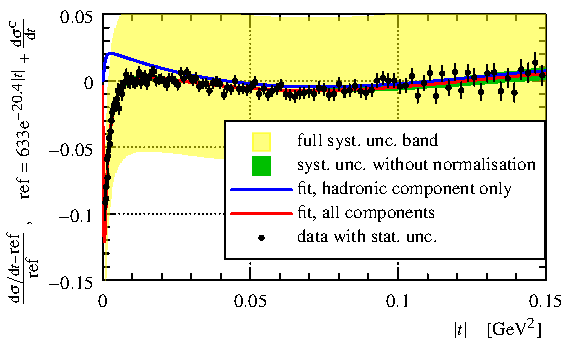
\includegraphics{fig/fit_details_exp3_0p15.pdf}
\vskip-2mm
\caption{%
Details of fit with $N_b = 3$ and $|t|_{\rm max} = 0.15\un{GeV^2}$.
}
\label{fig:fit exp3 0.15}
\end{center}
\end{figure}


\begin{figure}
\vskip-5mm
\begin{center}
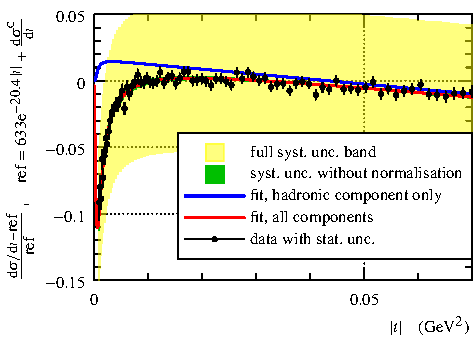
\includegraphics{fig/fit_details_exp1_0p07.pdf}
\vskip-2mm
\caption{%
Details of fit with $N_b = 1$ and $|t|_{\rm max} = 0.07\un{GeV^2}$.
}
\label{fig:fit exp1 0.07}
\end{center}
\end{figure}

The extreme cases in Table~\ref{tab:rho ref fits}, combination $N_b=1$ with $|t|_{\rm max} = 0.07\un{GeV^2}$ and $N_b=3$ with $|t|_{\rm max} = 0.15\un{GeV^2}$ have important meanings. In the latter, the largest possible sample is used and maximum flexibility is given to the fit. In that sense, this fit corresponds to the best $\rho$ determination considered. Also, in this case the fit data include many points where the CNI effects are limited. Consequently, the fit can ``learn'' the trend of the nuclear component and ``impose it'' in the region of strong CNI effects. Conversely, the fit configuration $N_b=1$ with $|t|_{\rm max} = 0.07\un{GeV^2}$ relies uniquely on data with sizeable CNI effects. This complementarity explains why these two cases give the extreme values of $\rho$ in Table~\ref{tab:rho ref fits}. Fit details for these two configurations are shown in Figures~\ref{fig:fit exp3 0.15} and \ref{fig:fit exp1 0.07}.

The fit configuration $N_b=1$ with $|t|_{\rm max} = 0.07\un{GeV^2}$ has another important meaning. Considering the shrinkage of the ``forward-cone'', this $|t|$ range is similar to the one used in the UA4/2 analysis \cite{ua4-rho}. This fact may suggest why UA4/2 could not observe deviations of the differential cross-section from pure exponential: the $|t|$ range was too narrow, as it would be for the present data, had the acceptance stopped at $|t| = 0.07\un{GeV^2}$, see Figure~\ref{fig:fit exp1 0.07}. Beyond the $|t|$ range, this fit combination shares more similarities with the UA4/2 fit (and in general with many other past experiments): purely exponential fit and assumption of constant hadronic phase. Moreover, as shown in Ref.~\cite{totem-8tev-1km}, the ``KL'' interference formula \cite{kl94} used in this report gives for this fit configuration very similar $\rho$ results as the ``SWY'' interference formula \cite{wy68} used in many past data analyses. From this point of this fit combination corresponds to the most fair comparison to previous $\rho$ determinations and their extrapolations, as e.g.~in Figure \ref{fig:rho_vs_s}. It is worth noting that this fit configuration yields a $\rho$ value incompatible at the level of about $4.7\un{\sigma}$ % (0.13663 - 0.09) / 0.01 = 4.663
with the preferred COMPETE model (blue curve in the figure).

\begin{figure*}
\vskip-5mm
\begin{center}
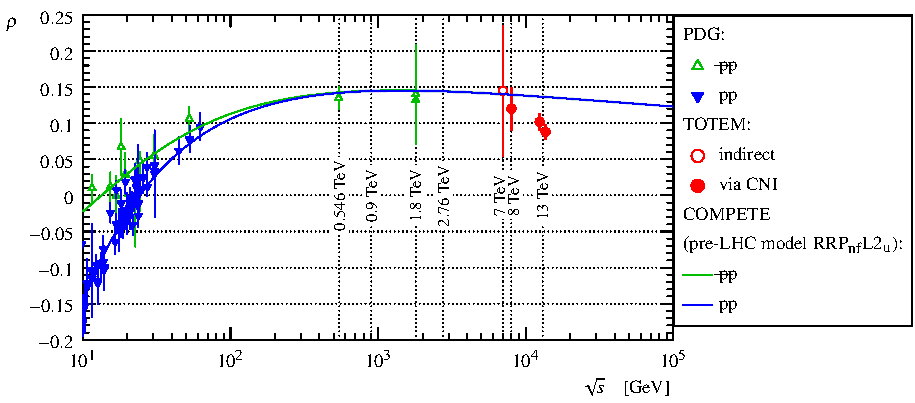
\includegraphics{fig/rho_vs_s.pdf}
\caption{%
Dependence of the $\rho$ parameter on energy. The $\rm pp$ (blue) and $\rm p\bar p$ (green) data are taken from PDG \cite{pdg-2010}. TOTEM measurements are marked in red. The two points at $13\un{TeV}$ correspond to the two selected fit cases discussed in text: the lhs.~point to the combination $N_b = 3$ and $|t|_{\rm max} = 0.15\un{GeV^2}$ while the rhs.~point to $N_b = 1$ and $|t|_{\rm max} = 0.07\un{GeV^2}$.
}
\label{fig:rho_vs_s}
\end{center}
\end{figure*}

Further tests were performed in order to probe the stability of the $\rho$ extraction. Since at higher $|t|$ values the effects of CNI are limited, one may conceive a two-step fit: first, use only the higher $|t|$ data to determine the parameters of the hadronic modulus, cf.~Eq.~(\ref{eq:nuc mod}), and second, optimise only $\rho$ with all the data but the hadronic modulus fixed from the first step. Figure~\ref{fig:fit exp3 0.15} indicates that for the first step one needs to include points down to about $|t| = 0.04\un{GeV^2}$ in order to describe correctly the concavity of the data. Performing the two-step fit with $N_b=3$ and with ansatz $\rho = 0.10$ (or $0.14$) yields, at the end, $\Delta\rho \approx 0.00$ (or $0.01$) wrt.~the standard $N_b=3$ fit presented above. Although for the ansatz $\rho = 0.14$ the result is somewhat larger (CNI effects cannot be fully neglected at higher $|t|$), these results demonstrate the pull of the data towards $\rho \approx 0.10$. A logical counterpart of the procedure just described would be to give the higher-$|t|$ data less weight. In its extreme, where the higher-$|t|$ data are not used at all, this has already been covered by fits with $|t|_{\rm max} = 0.07\un{GeV^2}$ discussed above.

\begin{figure*}
\vskip-5mm
\begin{center}
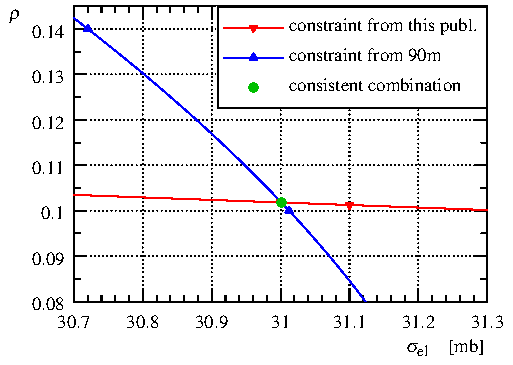
\includegraphics{fig/si_el_rho_solution.pdf}
\vskip-3mm
\caption{%
Constraints to the relation between $\rho$ and $\sigma_{\rm el}$ derived from this data set (red line) and from Ref.~\cite{totem-13tev-90m}. The solution consistent with both constraints is marked with a green dot.
}
\label{fig:si_el rho sol}
\end{center}
\vskip-2mm
\end{figure*}


Figure \ref{fig:si_el rho sol} illustrates a small correction due to a conceptual improvement in combining the data from this publication and from Ref.~\cite{totem-13tev-90m}. The latter assumes certain values of $\rho$ in order to evaluate cross-section estimates which are in turn used in this analysis (see Section~\ref{sec:normalisation}) to estimate $\rho$. This circular dependence can be resolved by considering simultaneously the $\rho$ dependence of $\sigma_{\rm el}$ in Ref.~\cite{totem-13tev-90m} (blue line) and the $\sigma_{\rm el}$ dependence of $\rho$ determined in this analysis (red line). The latter is done as linear interpolation of $\rho$ values extracted assuming $\sigma_{\rm el} = 30.9$ and $31.1\un{mb}$. The linear dependence is confirmed with Monte-Carlo studies. The solution consistent with both datasets (green dot) brings negligible correction to $\rho$ and $-0.03\un{\%}$ correction to the value of $\sigma_{\rm el}$ published in Ref.~\cite{totem-13tev-90m} for $\rho=0.10$.
